\documentclass[12pt,a4paper]{article}
\usepackage[a4paper,left=2cm,right=2cm,top=2cm,bottom=4cm]{geometry}
\usepackage[utf8]{inputenc}
\usepackage[T1]{fontenc}
\usepackage{amsmath}
\usepackage{babel}
\usepackage{amssymb}
\usepackage{float}
\usepackage{graphicx}
\usepackage{titling}

\usepackage{xcolor}
\usepackage{titlesec}



\definecolor{xsens}{RGB}{0,115,188}
\usepackage{sectsty}
%\chapterfont{\color{xsens}}  % sets colour of chapters
%\sectionfont{\color{xsens}}  % sets colour of sections
%\chapterfont{\color{xsens}}


\author{Mirco Huber}
\newcommand{\subtitle}{}
\title{Specifications BLE transmitter with TEDS sensors}


%%%%%%%%%%%%%%%%%% HEADER AND FOOTER
\usepackage{fancyhdr}
\setlength\headheight{40pt}
\renewcommand{\headrulewidth}{0pt}

\lhead{\thetitle}
\rhead{
\includegraphics[height=4em]{Logos/X-SENSORS-Logo_Slogan_EN_Transparent.png}}
\rfoot{\thepage}
\cfoot{}

\fancypagestyle{plain}{%
	\setlength\headheight{40pt}
	\renewcommand{\headrulewidth}{0pt}
	\lhead{\thetitle}
	\rhead{
\includegraphics[height=4em]{Logos/X-SENSORS-Logo_Slogan_EN_Transparent.png}}
	\rfoot{\thepage}
	\cfoot{}
	
}

\fancypagestyle{empty}{%
	\fancyhf{}
}

\usepackage{subfiles}

\titleformat{\chapter}[display]
{\normalfont\huge\bfseries}{}{0pt}{\thechapter.\ }

\usepackage{nicefrac}
\usepackage{tocloft}


\pagestyle{fancy}
\begin{document}
	\thispagestyle{empty}
	\begin{titlepage}
		\begin{figure}[H]
			\centering
			
\includegraphics[width=.5\linewidth]{Logos/X-SENSORS-Logo_Slogan_EN_Transparent.png}
		\end{figure}
		\vspace*{3cm}
		\begin{center}
			\Huge {\thetitle} \\\vspace*{.5cm}
			\small {\subtitle}
		\end{center}
		\vspace{12cm}
		\hspace{.6\linewidth} 
		\begin{tabular}{l}	
			\small{\theauthor} \\[.5pt]  
			\small{X-Sensors AG} \\ 
			\small{Landenbergerstrasse 13} \\
			\small{CH-8253 Diessenhofen} \\ [.5cm] 	
			\today
		\end{tabular}
	\end{titlepage}

	\setcounter{page}{1}
	\pagenumbering{arabic} % A-Z Seiten (werden ausgeblendet), geht nur um PDF
	\pagestyle{fancy}
	
	
	
	%%%%%%%%%%%%%%%%%%%%%%%%%%%
	\section{Initial situation}
	To maintain interchangeability between the sensors and transmitters, the calibration data for the sensors must be made available in an automated manner. Initially, we explored the possibility of providing this data through QR codes on the sensor's nameplate. However, due to the surface characteristics (cylindrical shell), these QR codes were not readily legible. As a result, we are now providing this data via TEDS. This approach offers the advantage of allowing the transmitter to directly transmit signals in their physical unit (kN) rather than in a ratiometric manner (mV/V).
	For this approach, two procedures need further specification:
	\begin{enumerate}
		\item Reading the calibration upon the transmitter's startup.
		\item Reading the calibration after sensor disconnection or exchange during the transmitter's runtime.
	\end{enumerate}
	\newpage
	\section{Reading calibration at startup}
	\begin{figure}[H]
		\centering
		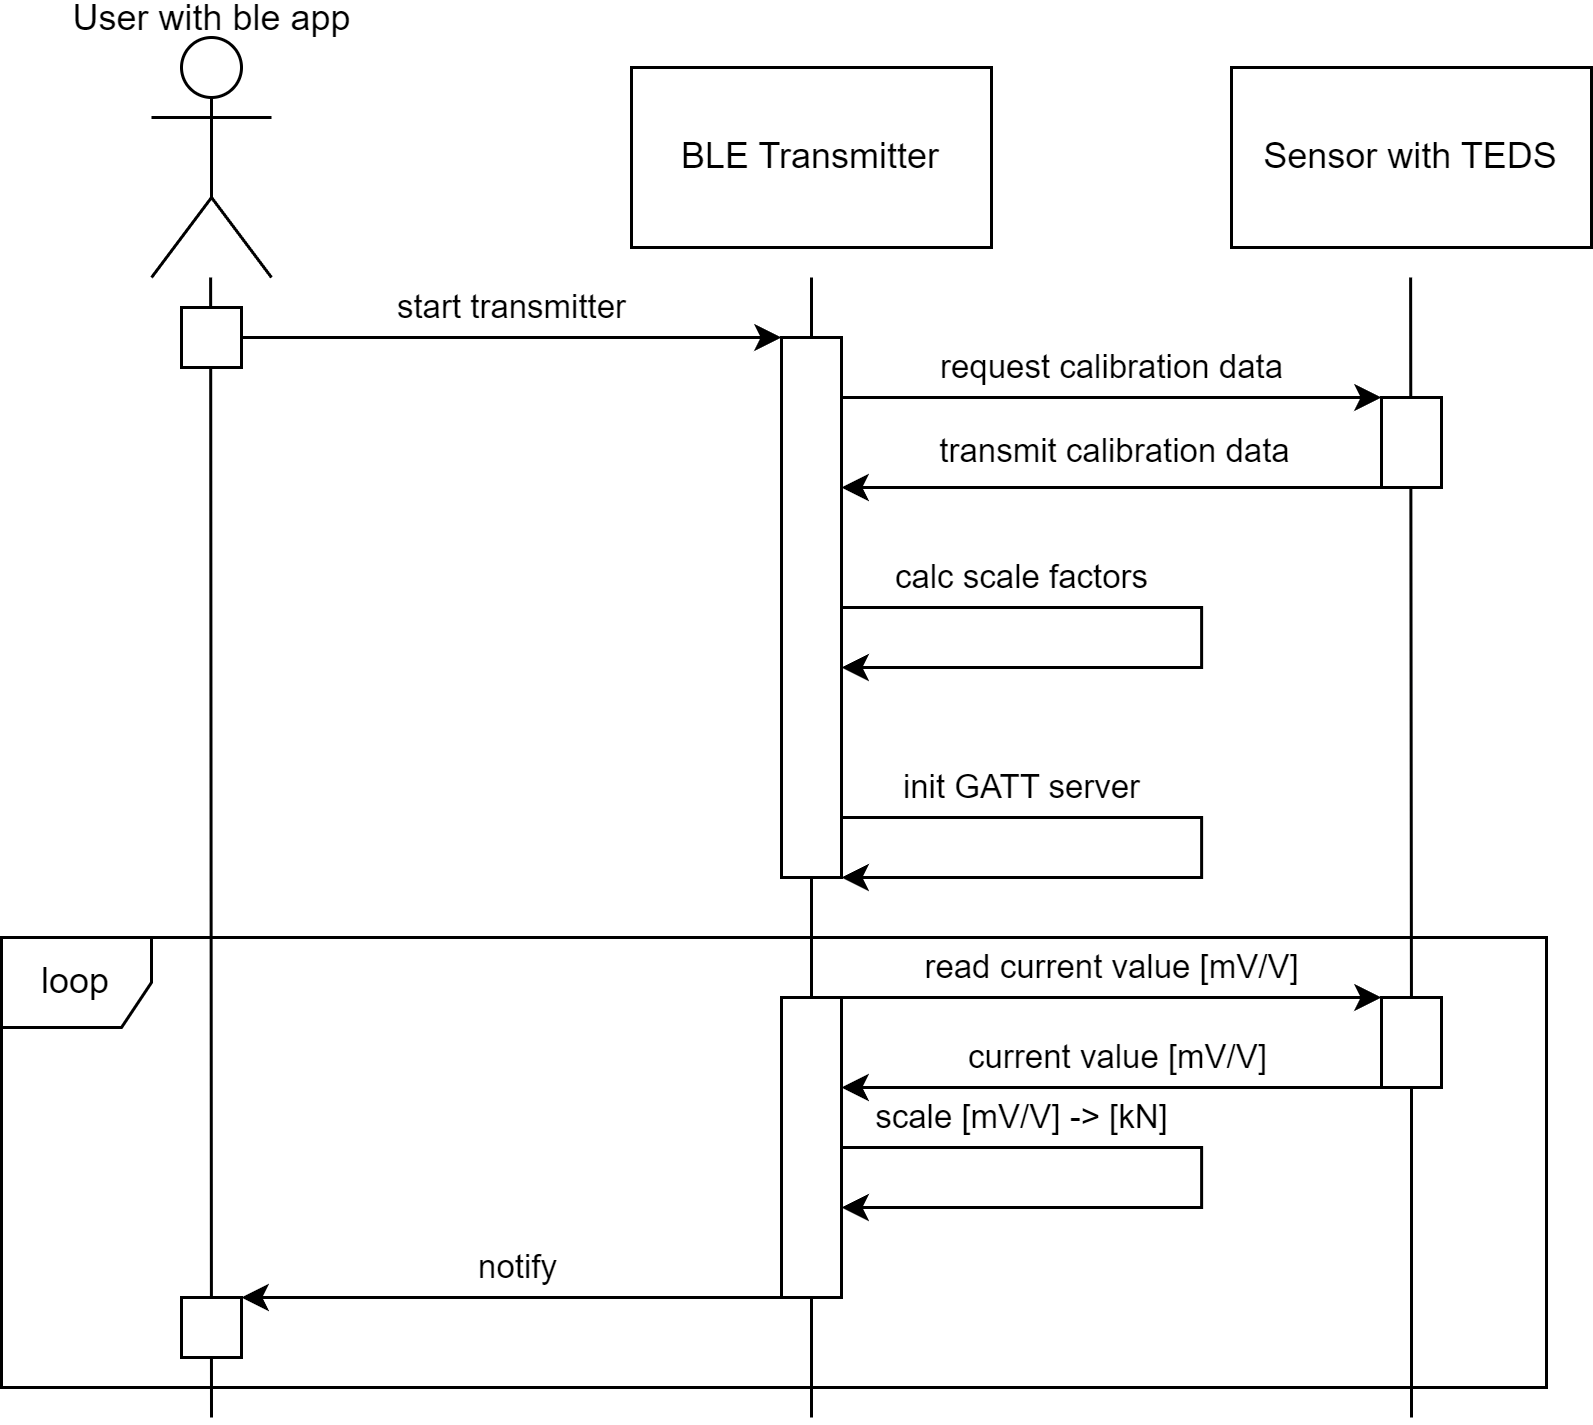
\includegraphics[width=1\linewidth]{C:/Users/Mirco/Downloads/calAtStartup}
		\caption{Sequence to read the calibration data at startup}
		\label{fig:calatstartup}
	\end{figure}
	\section{Reading calibration after change of setup}
	\begin{figure}[H]
		\centering
		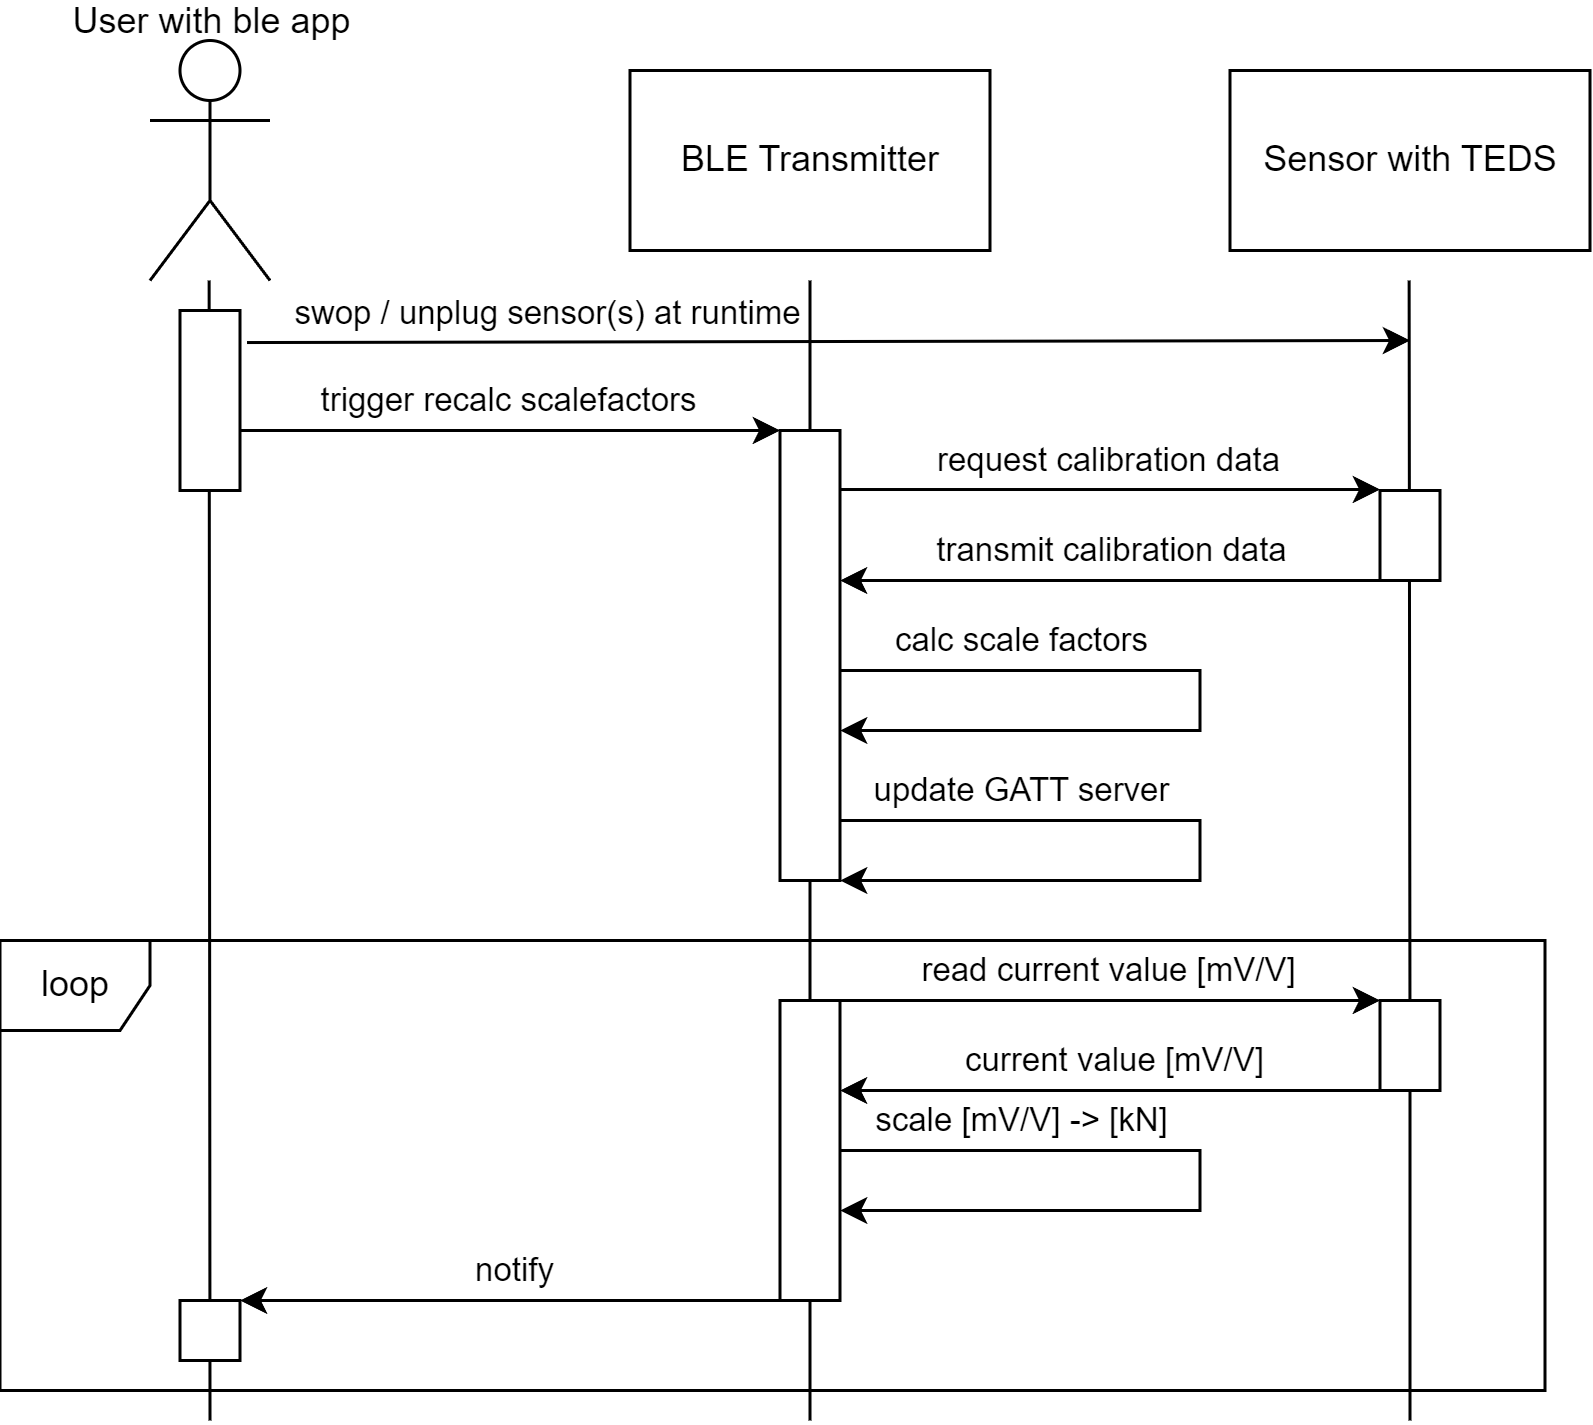
\includegraphics[width=1\linewidth]{C:/Users/Mirco/Downloads/calAfterSwop}
		\caption{Sequence to read the calibration data after swop/change}
		\label{fig:calafterswop}
	\end{figure}

	
%	\chapter{Erste Messkampagne vom 21.07.23}
%	\setcounter{page}{1}
%	\subfile{Teilberichte/Bericht_1/document}
%	\newpage
%	\chapter{Zweite Test Messkampagne vom 06.08.23}
%	\subfile{Teilberichte/Bericht_2/bericht}
%	\newpage
%	\chapter{Dritte Messkampagne vom 10.08.23}
%	\subfile{Teilberichte/Bericht_3/auswertung}
\end{document}